% !TEX encoding = UTF-8 Unicode

%% Document Details
\newcommand{\docTitle}{Spidergon Network-on-Chip}
\newcommand{\docAuthor}{Andrew Fecheyr Lippens}
\newcommand{\docDate}{\today}
\newcommand{\docSubject}{Redes en Chip}

% !TEX encoding = UTF-8 Unicode

\documentclass[12pt]{article}
\usepackage[utf8]{inputenc}
\usepackage[english]{babel}
\usepackage[pdftex]{graphicx}
\usepackage{fancyhdr}
\usepackage{url}
\newcommand{\HRule}{\rule{\linewidth}{0.5mm}}
\usepackage{geometry}
\usepackage[font=small,format=plain,labelfont=bf,up,margin=1cm]{caption}
\usepackage[pdftex,bookmarks=true,pdfborder={0 0 0},pdfauthor={\docAuthor},pdftitle={\docTitle},pdfsubject={\docSubject}]{hyperref}
\geometry{a4paper}

%% Set the document details
\title{\docTitle}
\author{\docAuthor}
\date{\docDate}

%% unbreakable words
\hyphenation{multi-core}

%%% BEGIN DOCUMENT
\begin{document}
\begin{titlepage}
\begin{center}
 
% Upper part of the page

\includegraphics[width=0.50\textwidth]{../shared/figures/logoUPV.pdf}\\[1cm]
\textsc{\LARGE Universidad Polit\'ecnica de Valencia}\\[1.4cm]
\textsc{\Large \docSubject}\\[1.4cm]
 
 
% Title
\HRule \\[0.4cm]
{ \huge \bfseries \docTitle}
\HRule \\[1.4cm]
 
% Author and supervisor
\begin{flushleft} \large
\emph{Author:}\\
\docAuthor
\end{flushleft}

\vfill
 
% Bottom of the page
{\large \docDate}
 
\end{center}
\end{titlepage}

\begin{abstract}
	\todo[write an abstract]
\end{abstract}

\setcounter{tocdepth}{2}
\begin{tableofcontents}
\end{tableofcontents}

\newpage

\section{Introduction}\label{C:intro}
	
	A network-on-chip or NoC has become one of the key components in digital chips. As the number of components and transistors per chip grows continuously, most chips have become multi-core. These chips consist of a number of separate cores, often with fixed-function accelerators, memory arrays and input/output units.
		
	Historically buses or crossbar switches were used to connect the functional components of a chip. Above four cores, however, the limited bandwidth of a bus becomes a major limitation, and above 8 or 16 cores, crossbar switches become very expensive. Only a NoC provides the scalability needed for emerging multicore chips. The NoC bounds the performance potential of these chips and accounts for a substantial fraction of the power and area consumption.

\subsection{Technical Terms}\label{S:terms}
	This paper uses technical terms from the domain of computer networks. Some of them are explained here to help the reader.

\begin{description}

\item[System on Chip (SoC)] 
	refers to the integration of all components of a computer or electronic system into a single integrated circuit (chip).\cite{wikiSoC}
	
\item[An Interconnect Processing Unit (IPU)] 
	is essentially an on-chip communication network with hardware and software components which jointly implement key functions of different SoC programming models through a set of communication and synchronization primitives and provide low-level platform services to enable advanced features in modern heterogeneous applications on a single die.\cite{coppola2008design}

\item[A Chip multiprocessor (CMPs)] is a multi-core processor in which the distinct cores are integrated onto a single integrated circuit die.

\end{description}

\section{Bus vs. Network-on-Chip}\label{C:busvsnoc}

\section{Spidergon Topology}\label{C:topology}
	\begin{figure}[ht]
	\centering
		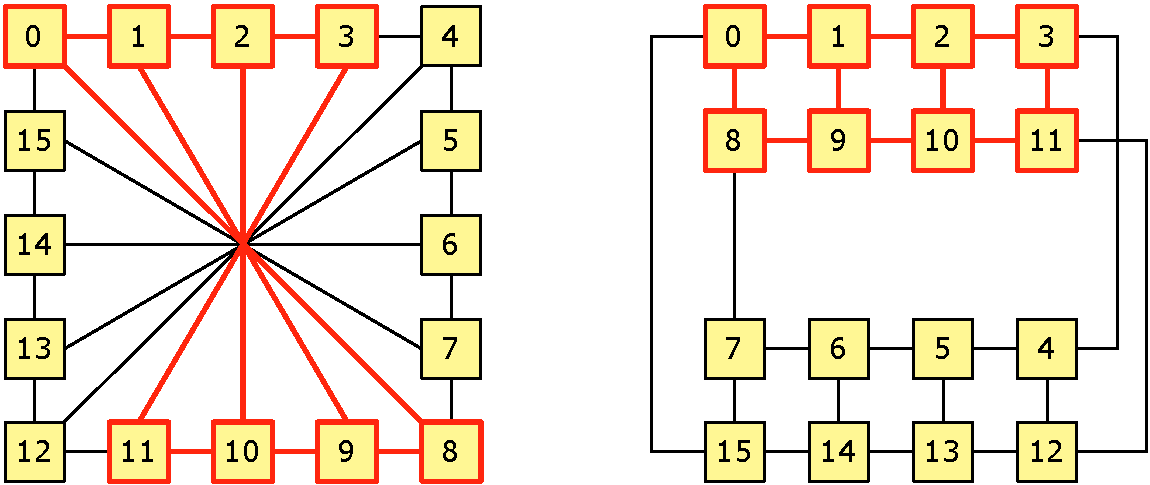
\includegraphics[width=0.75\textwidth]{topology3}
		\caption{Equivalent representation of Spidergon STNoC for ${N}$ = 16}
		\label{fig: topology}
	\end{figure}

\section{Conclusion}\label{S:conclusion}
	\todo

\bibliographystyle{plain}
\bibliography{spidergon}

\end{document}

